\documentclass[a4paper,10pt,oneside]{scrreprt}
\usepackage[latin1]{inputenc}
\usepackage[english]{babel}
\usepackage{graphicx}
\usepackage{float}
\usepackage{geometry}
\geometry{verbose,a4paper,tmargin=15mm,bmargin=25mm,lmargin=15mm,rmargin=15mm}
\usepackage{paralist}

\usepackage{paracol}

\usepackage{todonotes}

\usepackage{listings}
\lstset{language=Java,
	tabsize=2,
	showspaces=false,
	showtabs=false,
	breaklines=true,
	showstringspaces=false,
	breakatwhitespace=true,
	commentstyle=\color{pgreen},
	keywordstyle=\color{pblue},
	stringstyle=\color{pred},
	basicstyle=\footnotesize\ttfamily,
	moredelim=[il][\textcolor{pgrey}]{$$},
	moredelim=[is][\textcolor{pgrey}]{\%\%}{\%\%}
}

\usepackage{tikz}
\usetikzlibrary{calc,patterns,angles,quotes}

\usepackage{caption}
\usepackage{subcaption}
\usepackage{tabularx} % in the preamble

\usepackage{pdfpages}

%\usepackage{indentfirst} % for always indenting the first paragraphs

\usepackage{wrapfig}
\usepackage{lipsum}
\usepackage[linewidth=1.2pt,linecolor=red]{mdframed} % for boxes around wrapfigure and text

\begin{document}


\begin{center}
	Submitted by Group 18

	\bigskip

	\begin{tabular}{c}
	Group Members: \\
	CETIN, Ulfet (391819); GRUCZKA, FILIP (413279);	LIPINSKI, Bartosz (413177) \\
	SZYMANSKI, Bartosz (411949); GONG, Zeheng (378125)\\
	\end{tabular}

	\bigskip

	DIS1 WS 19/20 - Project Milestone III\\
	Ideation - Phase II\\

	%	(ordered on lastname basis)
\end{center}
\vspace{-1cm}

\clearpage

\begingroup
\let\clearpage\relax
	\chapter{Storyboard walkthrough}
\endgroup


\section{Solution \#1:}

\begin{figure}[H]
	\centering
	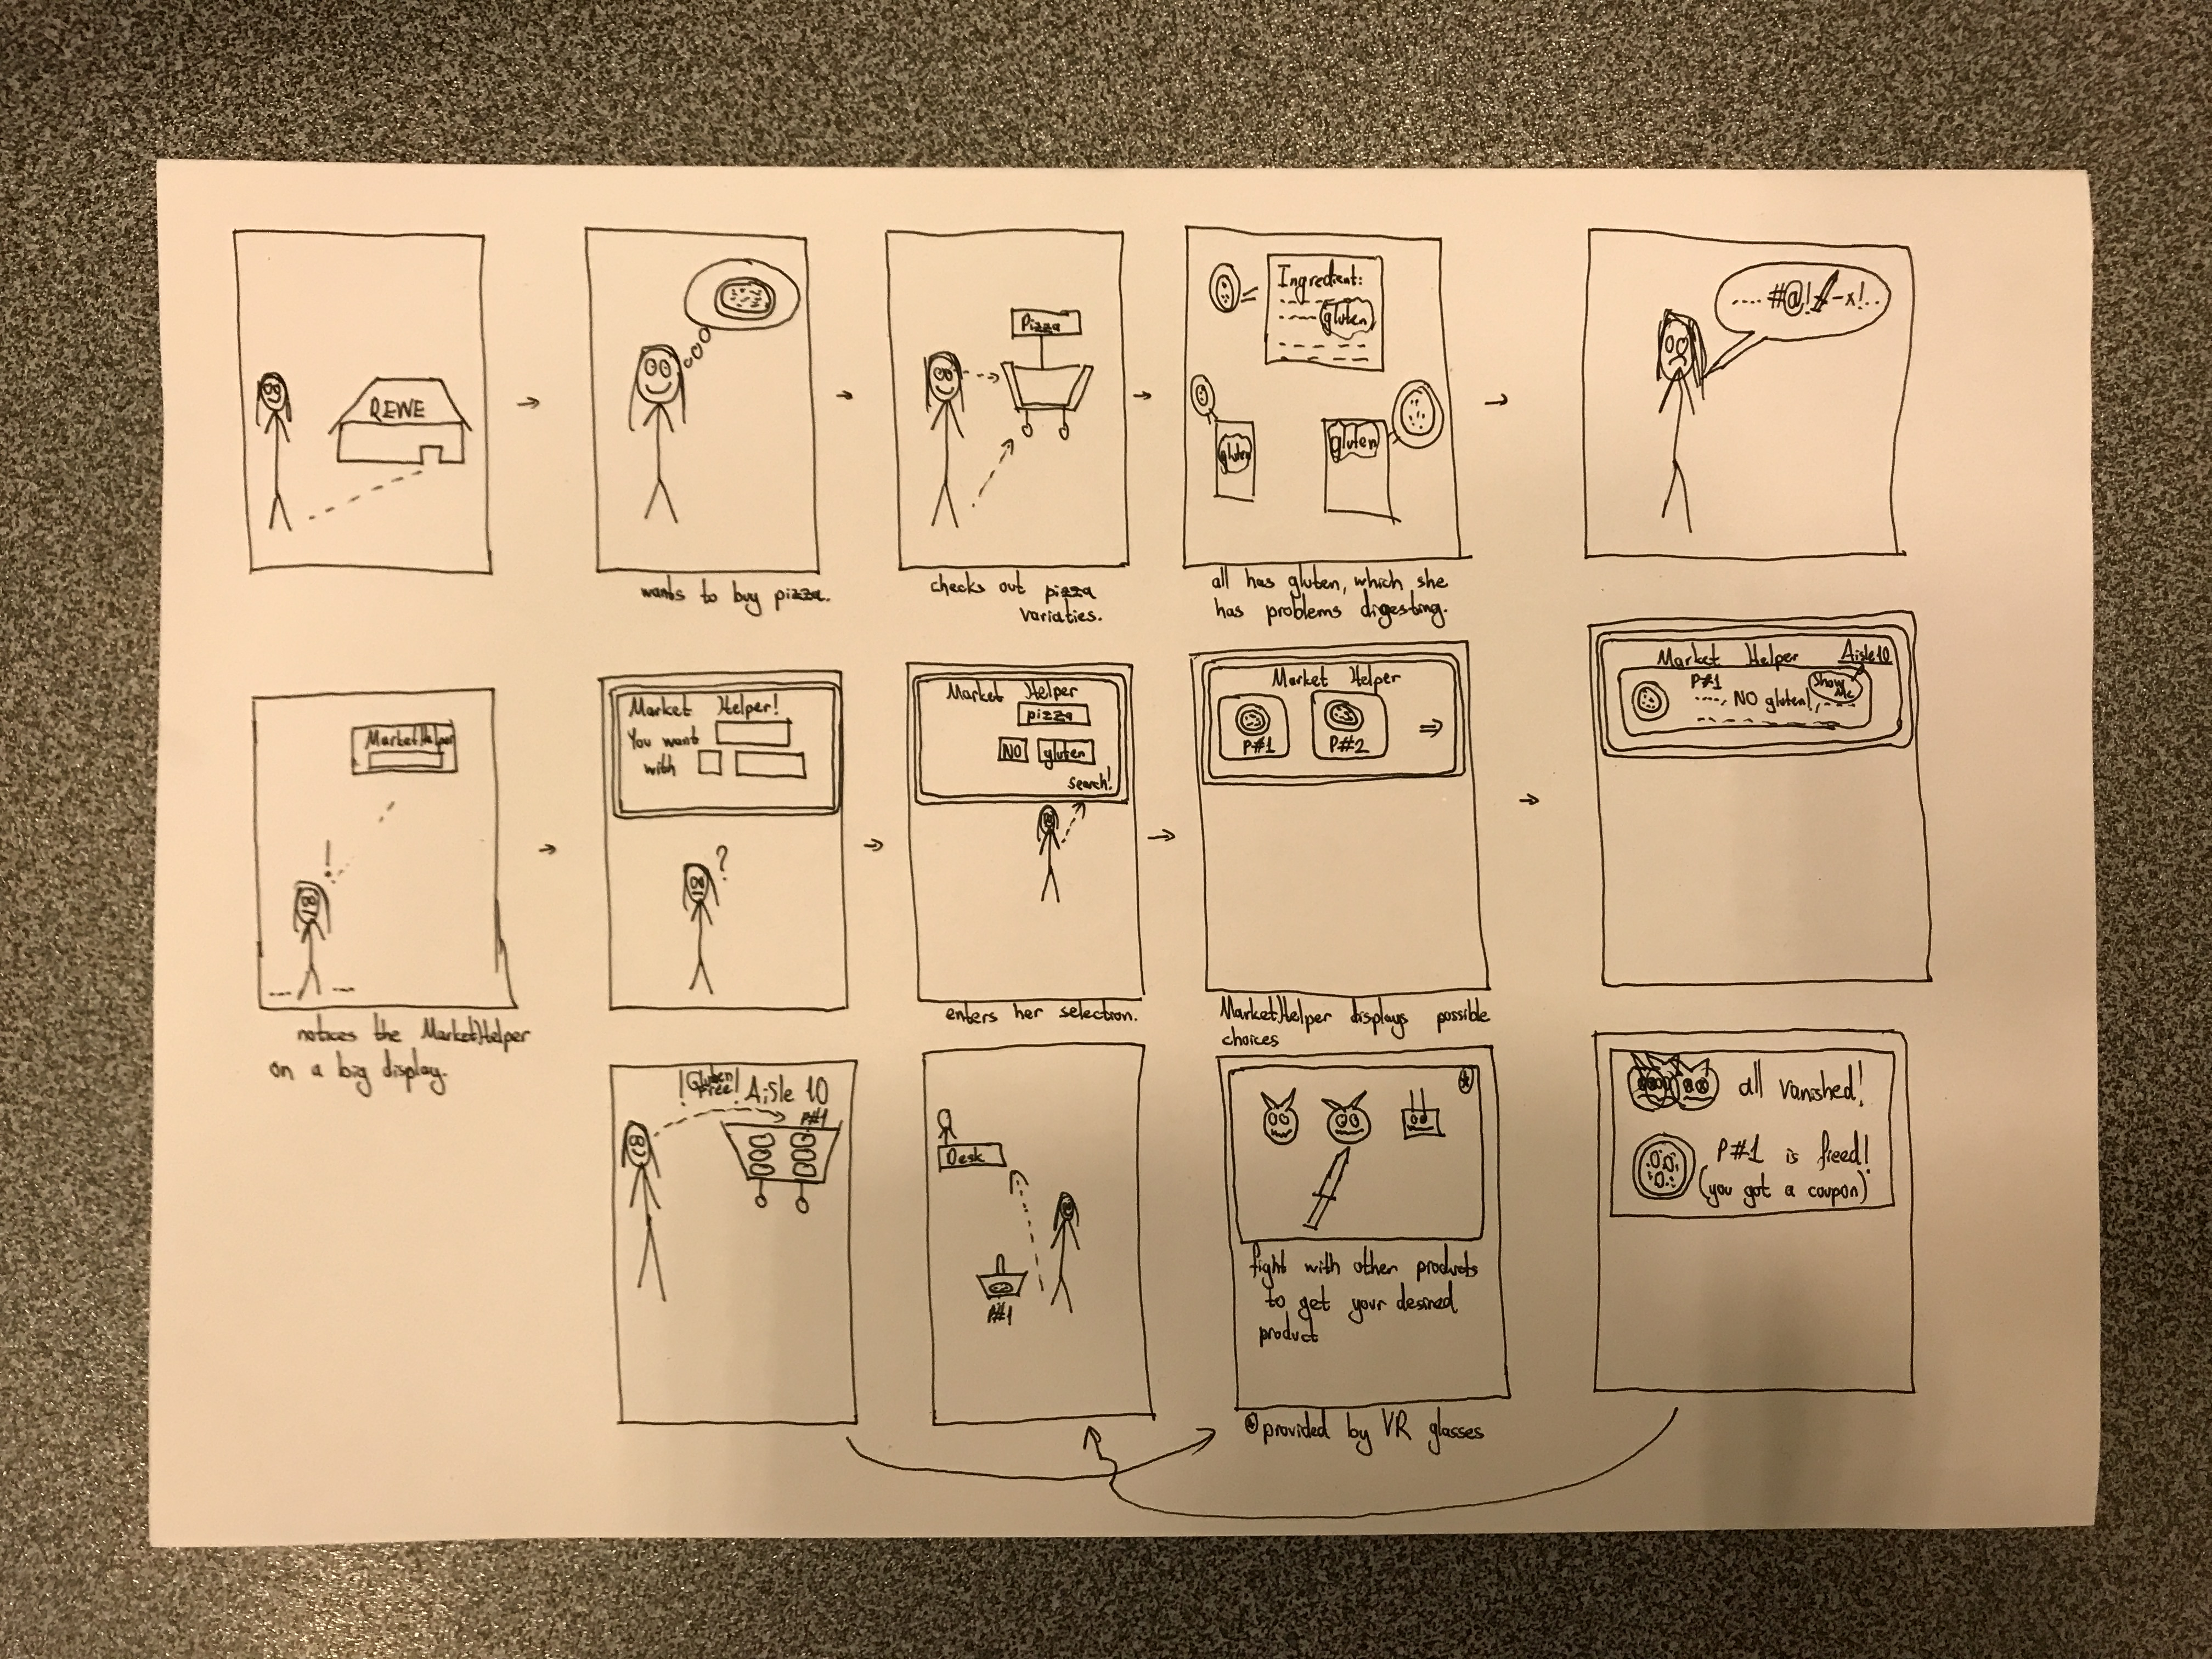
\includegraphics[scale=0.16, clip, trim={40em 28em 40em 33em}]{images/s1.jpg}
\end{figure}

User \#1:
\begin{compactitem}
	\item Name: Hakan
	\item Information: age of 23, Turkish
	\item Profession: M.Sc. student
	\item likes to  play games and hang out with friends
	\item representative of our third persona (David)
\end{compactitem}
\bigskip

Answers:
\begin{compactitem}
	\item Do the users understand the solution?\\
		Yes, it was clear for the user. The user also really likes the solution.\\
	
	\item Do the users find the solution realistic?\\
		Not so much. The other parts are really possible, while VR goggles part was not realistic at all: the fighting with the other mascots is silly, not everyone wants that (might be hard for elderly). But fighting for right-earned food might also be fun for some.\\
		
	\item Do the users feel that this solution can solve his/her problem(s)? If not, what is still
	a problem? Is there a solution that could solve this?\\
		Yes, especially when he wants to find some obscure ingredient that he needs to complete a recipe. It is also better than asking some retail worker. He agreed that it might solve his problem.
\end{compactitem}
\bigskip

Transcript of the User Study (shortened):\\

\noindent Q: (the solution is explained) Can you take a look first? On the first box you can see a girl, this girl has a specific condition, ..., she has to find a specific product (pizza with no gluten), yet it does not have to be about just some health condition.  \\
A: It is pretty clear from the drawings and also after you explained. I think it is a quite nice solution.\\
Q: Do you find the solution realistic?\\
A: To be honest, the part about VR goggles are not really realistic, but the parts before are quite realistic and possible. \\
Q: Why do you think so?\\
A: The fighting with the other mascots are for me silly, people do not want to fight each time they go shopping. Also, not good for elderly, for example, and it seems kinda silly.\\
Q: Do you think that people would find this fun? Did you find this idea fun?\\
A: It could be fun, yeah. You can just get into the game (like role-playing) and in the end, you get your hard earned food, but I do not think it is a viable solution here.\\
Q: Do you have such a problem (of finding the right food)\\
A: (explains his experience, especially about specific recipes calling for specific ingredients) This kind of thing would help. So yes.


\bigskip
\bigskip

User \#2:
\begin{compactitem}
	\item Name: Furkan
	\item Information: age of 26, Turkish
	\item Profession: M.Sc. student
	\item interested in fitness, likes to learn about anything, joining online courses, gym-going, reading a lot
	\item representative of our first persona (Picky Eater Helga Ratt)
\end{compactitem}
\bigskip

Answers:
\begin{compactitem}
	\item Do the users understand the solution?\\
		Yes, only the game part is not very clear. How is he going to kill the other mascots was not clear. One other question was whether VR goggles are going to provided by the market.\\
	
	\item Do the users find the solution realistic?\\
	He is both concerned about the number of available screens in the market and who would provide the VR goggles. In short, he does not find it that much realistic.\\
	
	\item Do the users feel that this solution can solve his/her problem(s)? If not, what is still
	a problem? Is there a solution that could solve this?\\
		He thinks this would not solve his problems in its current form. He would like to have it in a way that more than one item is searchable via the application, so we would not spend so much time in front of the screen. However, he finds this promising.\\
		(he is also curious whether people would be concerned about gazes of others, as this application would be out in the open and everyone would see what he searched for)\\
		He said playing games in home and coming to fetch the coupons would be more fun!
\end{compactitem}
\bigskip

User \#3:
\begin{compactitem}
	\item Name: Sare
	\item Information: age of 27, Turkish
	\item Profession: M.Sc. student in Industrial Engineering
	\item spending time with friends, doing sports, reads a lot, loves traveling around, cooks a lot  
	\item representative of our mother persona (due to her cooking a lot)
\end{compactitem}
\bigskip

Answers:
\begin{compactitem}
	\item Do the users understand the solution?\\
	The user understood the solution. She thinks that it would help especially when she checks whether some product has pork in it.\\
	
	\item Do the users find the solution realistic?\\
	Yes, but the cost of such VR peripherals seems a bit high to her.\\
	
	\item Do the users feel that this solution can solve his/her problem(s)? If not, what is still
	a problem? Is there a solution that could solve this?\\
	She believes that this could solve her problem, but something that would take her to the actual place might help better.\\
	
\end{compactitem}

\clearpage

\section{Solution \#2:}
\begin{figure}[h]
	\centering
	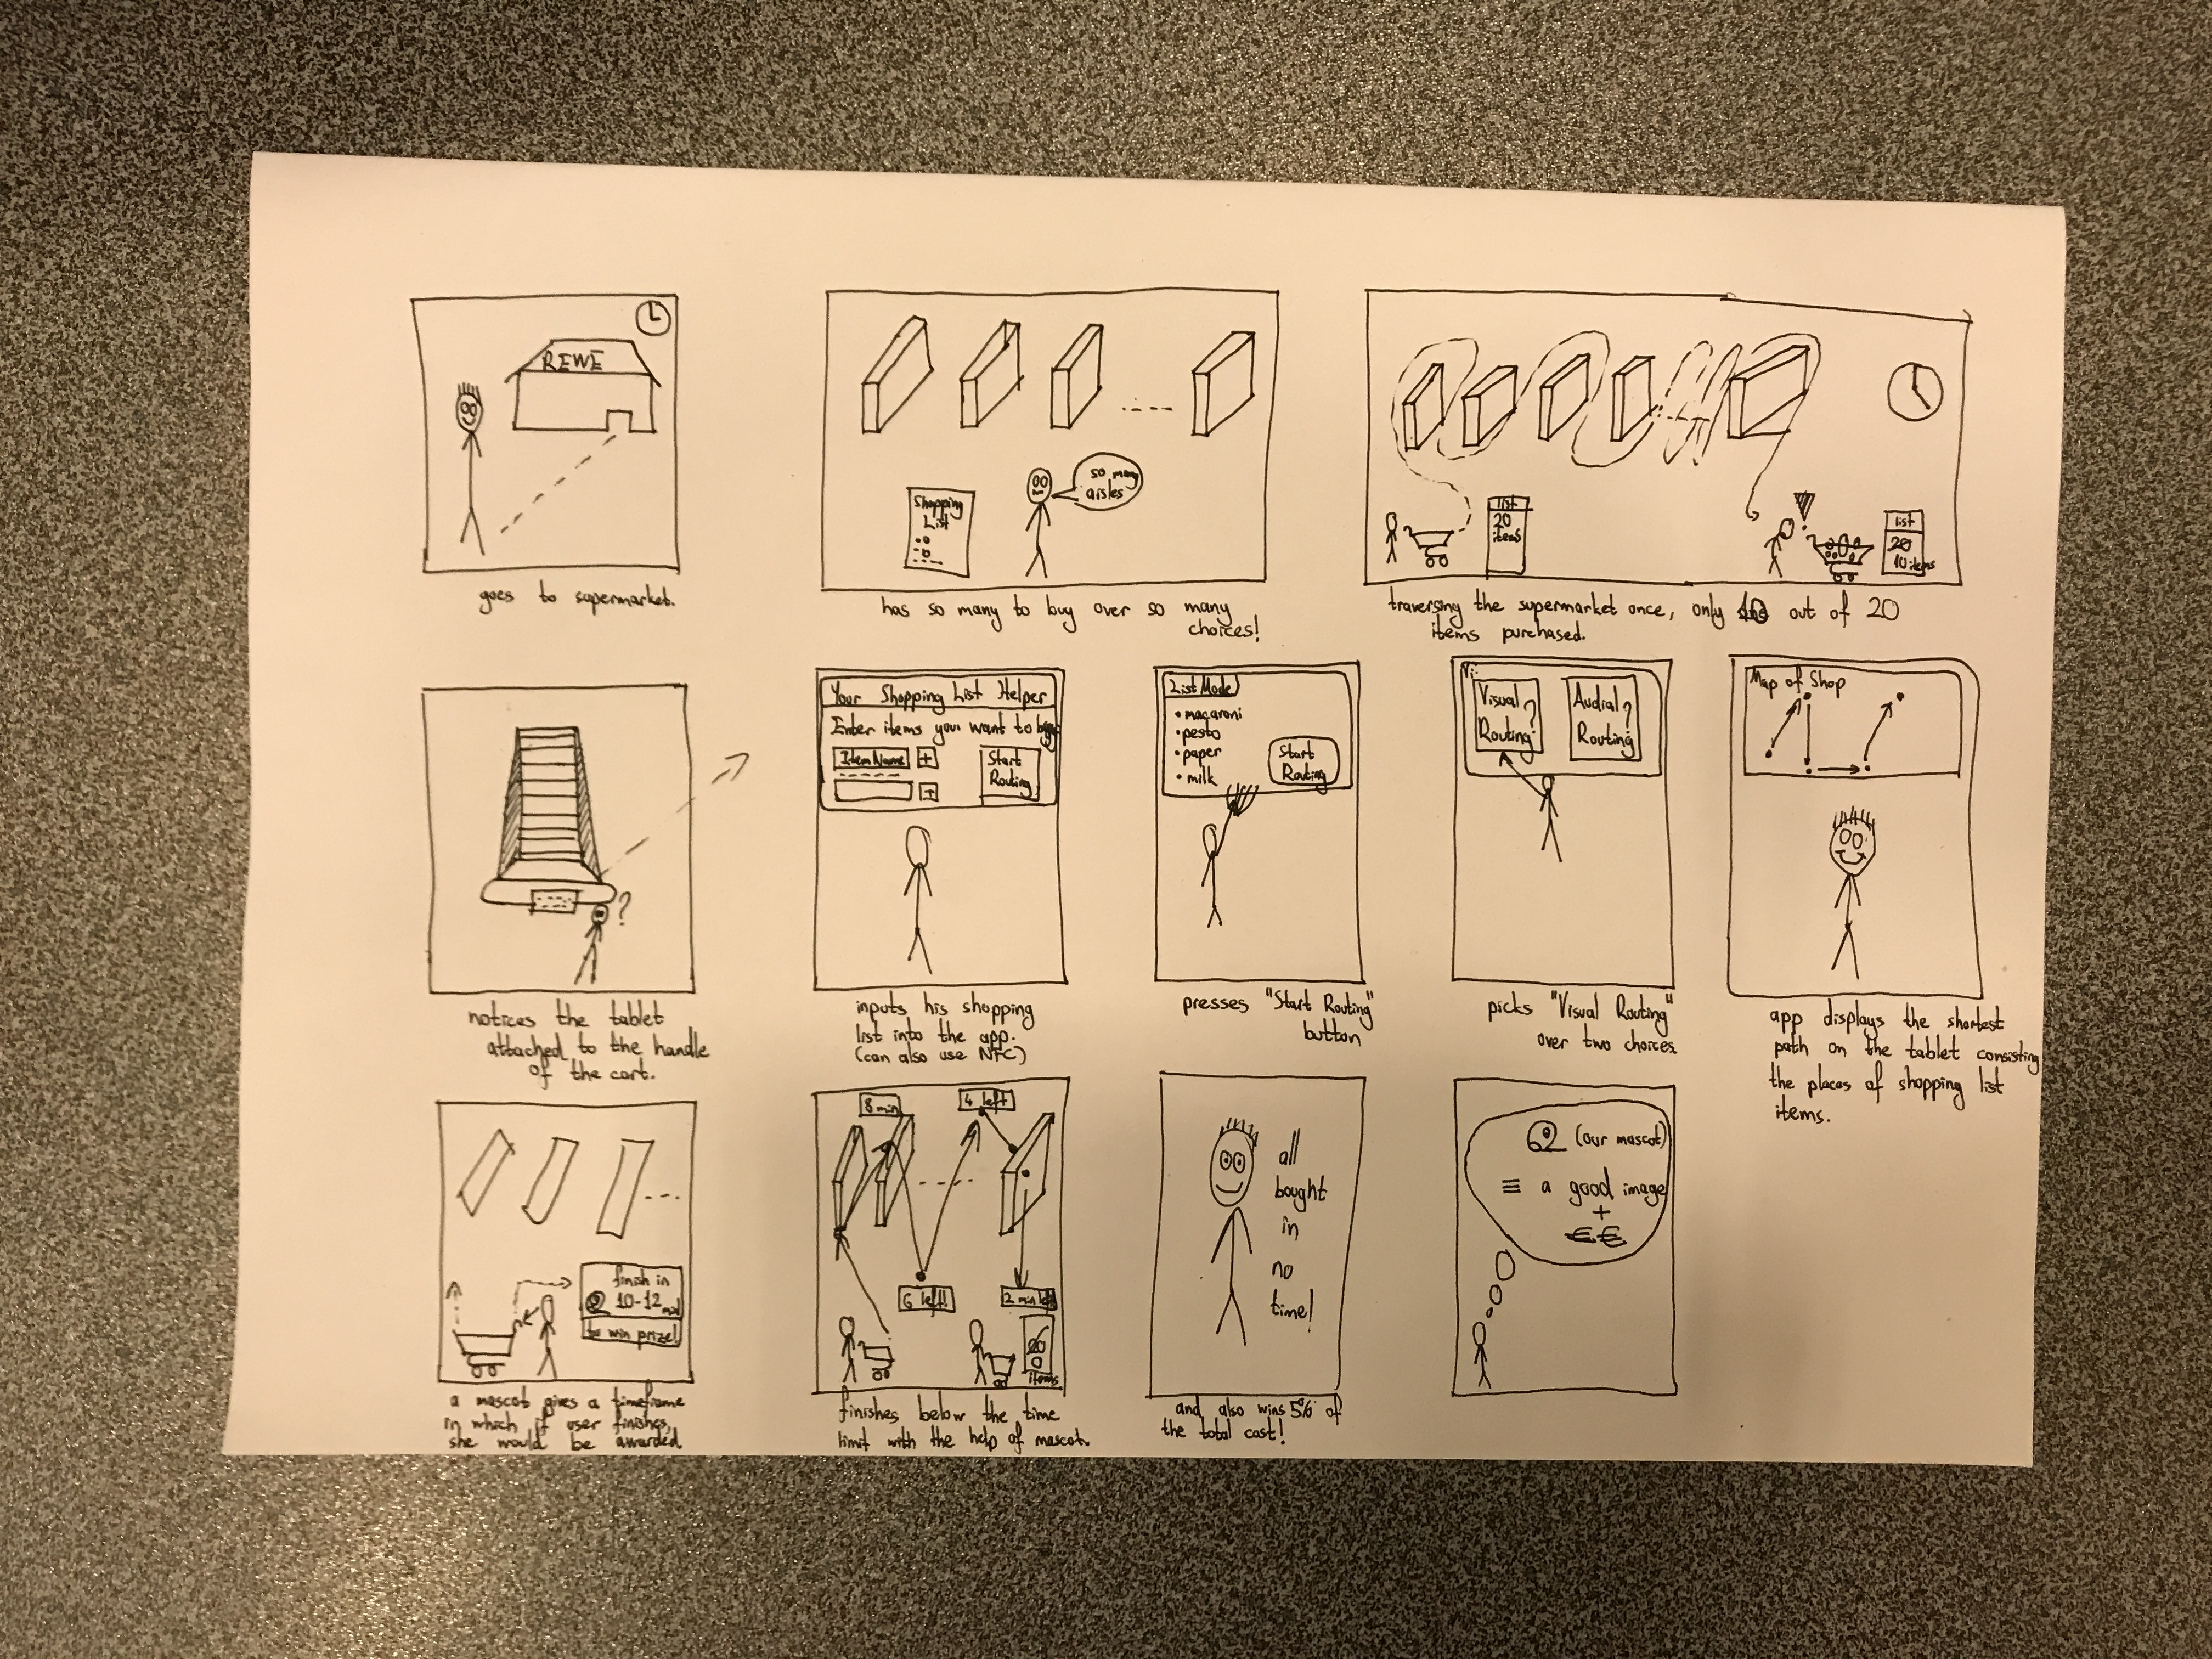
\includegraphics[scale=0.16, clip, trim={71em 35em 33em 43em}]{images/s2.jpg}
\end{figure}

User \#1:
\begin{compactitem}
	\item Name: Hakan
	\item Information: age of 23, Turkish
	\item Profession: M.Sc. student
	\item likes to  play games and hang out with friends
	\item representative of our third persona (David)
\end{compactitem}
\bigskip

Answers:
\begin{compactitem}
	\item Do the users understand the solution?\\
	Yes, it is quite clear. The user were able to explain the solution completely by putting himself in the shoes of the example in the storyboard.\\
	
	\item Do the users find the solution realistic?\\
	Much more realistic than the Solution \#1. Also, he finds this solution innovative to come up with.\\
	
	\item Do the users feel that this solution can solve his/her problem(s)? If not, what is still
	a problem? Is there a solution that could solve this?\\
	Yes, definitely. He also goes around the shop and got bored afterwards seeing all the same places, and this would really improve his experience.\\
\end{compactitem}
\bigskip

\noindent Q: (solution explained) The storyboard is a bit obscure (the candidate agrees). You can choose a routing based on your preference. (...) In a time range, if the customer goes to the cash desk, with the mascot cherishing for you. Do you understand the solution?\\
A: Yes, quite clearly. (the user explains in a short manner)\\
Q: Do you find the solution realistic?\\
A: Yes, especially compared to the solution \#1. As long as the layout of the shop significantly changes, it is pretty innovative thing to come up with.\\
Q: Do you find the solution fun?\\
A: Yes, unlike the first one, it does not interfere with my shopping, and if I am fast enough, and with a coupon that is a positive feedback, that is actually pretty good.\\
Q: (some extra questions on usability)


\bigskip
\bigskip

User \#2:
\begin{compactitem}
	\item Name: Furkan
	\item Information: age of 26, Turkish
	\item Profession: M.Sc. student
	\item interested in fitness, likes to learn about anything, joining online courses, gym-going, reading a lot
	\item representative of our first persona (Picky Eater Helga Ratt)
\end{compactitem}
\bigskip

Answers:
\begin{compactitem}
	\item Do the users understand the solution?\\
	Yes, user understands the solution and can explain the solution with his own words.
	\\
	
	
	\item Do the users find the solution realistic?\\
	Yes, but the user finds it not so viable for the supermarket, as supermarkets want the customers to spend more time inside, so the customers would buy more.
	\\
	
	\item Do the users feel that this solution can solve his/her problem(s)? If not, what is still
	a problem? Is there a solution that could solve this?\\
	Yes, the user agrees that this product would solve his problem, yet he is curious about the approaches of the supermarkets towards this product. Moreover, he does not want to be seen running around for coupons (it is explained that there would be time frame, so no early finishers would be gifted coupons)
	\\
\end{compactitem}
\bigskip

\noindent Q: (solution explained as before) \\
A: (finds the mascot not decipherable, explains the solution in his words) \\
Q: Do you find the solution realistic?\\
A: Realistic, but one catch: there is a product like that. It is also counterproductive in the sense of supermarket, they want people to spend money. Good for the customer, not so good for the supermarket.\\
Q: Do you think that this solution can solve your problem?\\
A: Definitely. Would help me in my shopping, no doubt.\\
Q: Would it be more fun? \\
A: Nobody would like to look cheap running around (we explained that there would be a timeframe, not would be a race to go earlier)\\

User \#3:
\begin{compactitem}
	\item Name: Sare
	\item Information: age of 27, Turkish
	\item Profession: M.Sc. student in Industrial Engineering
	\item spending time with friends, doing sports, reads a lot, loves traveling around, cooks a lot  
	\item representative of our mother persona (due to her cooking a lot)
\end{compactitem}
\bigskip

Answers:
\begin{compactitem}
	\item Do the users understand the solution?\\
	She understood the solution and she was able to explain the solution in her own words in 5 sentences. She finds the solution very enjoyable.\\
	
	
	\item Do the users find the solution realistic?\\
	She finds the solution realistic, and she thinks this should be implemented in supermarkets.\\
	
	\item Do the users feel that this solution can solve his/her problem(s)? If not, what is still
	a problem? Is there a solution that could solve this?\\
	That would definitely solve her problem, as she spends most of her time traveling around a supermarket.\\
\end{compactitem}
\bigskip



\clearpage
\section{Solution \#3:}


\begin{figure}[H]
	\centering
	\includegraphics[scale=0.10, clip, trim={0em 0em 0em 0em}]{images/s3.jpg}
\end{figure}


User \#1:
\begin{compactitem}
	\item Name: Maria
	\item Information: age of 43, Polish, mother of 3 young kids
	\item Profession: teacher
	\item representative of our mother persona
\end{compactitem}
\bigskip

Answers:
\begin{compactitem}
	\item Do the users understand the solution?\\
	In general she understood the solution. The only one problem what made her confused was possibility to try different dishes. She described that storyboard shows "normal" size dish instead of little portion to try. I had to clarify that main idea is to get inspiration what to cook.\\
	
	
	\item Do the users find the solution realistic?\\
	She is around 40 years old and she is not technological geek. So didn't get valuable response. She just said "Yeah why not, that will be beneficial for users and supermarkets Such solution will definitely attract people."\\
	
	\item Do the users feel that this solution can solve his/her problem(s)? If not, what is still
	a problem? Is there a solution that could solve this?\\
	She really like this solution. "I'm always tired and bored after 8 hours of work. Before relaxing in the front of TV i have to do everyday shopping.". The only one aspect what made her confused, was that even though after relaxing in the massage chair she has to cook at home. She said "What about - buying HEALTHY dishes in supermarket? I can imaging reading my favourite book in the store and someone else is preparing food for me. But it has to be healthy and well prepared. Then I will be able even to pay little bit more. Yeah that sounds better. I will pick what my family wants to eat and then I will have 30 min of relax."
\\
\end{compactitem}
\bigskip

User \#2:
\begin{compactitem}
	\item Name: Marek
	\item Information: age of 23, Polish
	\item Profession: Computer Science student
	\item representative of our student persona
\end{compactitem}
\bigskip

Answers:
\begin{compactitem}
	\item Do the users understand the solution?\\
	He understood the solution, and he explained storyboard correctly. He had just one idea for improvement "I don't see sense of making
parallel stories. One story without your system and one with your system. I think better will be focus on yours system, and not show how ordinary shopping look - everyone know that."\\
	
	\item Do the users find the solution realistic?\\
	He was really pessimistic about the solution. He was complaining about the price and target users. "Firstly that will be extremely expensive to implement. Whole supermarkets will have to have 
larger dimensions.. System itself will be expensive. If you will provide 10 massage chairs. What about other people waiting for massage? Maybe better will be to called it "Massage and food" and provide something like restaurant. And skip the concept of implementing it in supermarkets."\\
	
	\item Do the users feel that this solution can solve his/her problem(s)? If not, what is still
	a problem? Is there a solution that could solve this?\\
	He said that it will be nice improvement in shopping. But as mentioned earlier - hard to implement. \\
\end{compactitem}
\bigskip

User \#3:
\begin{compactitem}
	\item Name: Agata
	\item Information: age of 20, Polish
	\item Profession: Law student
	\item representative of our picky eater persona
\end{compactitem}
\bigskip

Answers:
\begin{compactitem}
	\item Do the users understand the solution?\\
	She understood the solution. She could explain storyboard step by step.\\

	\item Do the users find the solution realistic?\\
	She was optimistic about the solution. But she was rather thinking about "nice solution for her problem" and she was not deep thinking about other aspects as price and actual implementation.\\

	\item Do the users feel that this solution can solve his/her problem(s)? If not, what is still
	a problem? Is there a solution that could solve this?\\
	She said that our solution will be helpful for her if - "You will serve products without lactose for me. Then I'll find solution to my problems with finding products in supermarkets"\\
\end{compactitem}

\clearpage
\section{Solution \#4:}
\begin{figure}[h]
	\centering
	\includegraphics[scale=0.16, clip, trim={71em 35em 33em 43em}]{images/s4.jpg}
\end{figure}
User \#1:
\begin{compactitem}
	\item Name: Magda
	\item Information: age of 47, Polish
	\item Profession: accountant 
	\item a mother of two
	\item representative of our mother persona 
\end{compactitem}
\bigskip

Answers:
\begin{compactitem}
	\item Do the users understand the solution?\\
		Yes, the user did understood the solution and she was able to correctly explain solution by herself.\\
	
	\item Do the users find the solution realistic?\\
		Even though she isn't a technological geek, she found realistic since the solution uses an app and screen on refrigerator, similiar to the one she has at her home.\\
		
	\item Do the users feel that this solution can solve his/her problem(s)? If not, what is still
	a problem? Is there a solution that could solve this?\\
		User opinion is that she thinks it would be great to encourage kids to buying healthy food and she would love some help with planning what to buy, 
but she isn't entirely convinced that most kids would enjoy cartoons about healthy food. In general, she feels that this solution would solve her problems
if cartoons were entertaining for kids

\end{compactitem}
\bigskip
\bigskip
User \#2:
\begin{compactitem}
	\item Name: Jan
	\item Information: age of 21, Polish
	\item Profession: undergraduate student in Poland
	\item philology student
	\item representative of our student persona 
\end{compactitem}
\bigskip

Answers:
\begin{compactitem}
	\item Do the users understand the solution?\\
		Yes, he did understood it correctly.\\
	
	\item Do the users find the solution realistic?\\
		Yes, he found it realistic. However, he noted that making cartoons requires a lot of time, creative people and money.\\
		
	\item Do the users feel that this solution can solve his/her problem(s)? If not, what is still
	a problem? Is there a solution that could solve this?\\
		He stated that he would like some help with his desire to eat healthy and any app that helps and reduces time spend in shop is good, but he feels that this solution
isn't suited for him, even though he has little sister. However, he can imagine, that it might be helpful for him in the future, when he'll become a parent.

\end{compactitem}
\bigskip
\bigskip
User \#3:
\begin{compactitem}
	\item Name: Kacper
	\item Information: age of 21, Polish
	\item Profession: undergraduate student in Great Britain
	\item electronics student and marathon runner
	\item representative of our picky eater persona
\end{compactitem}
\bigskip

Answers:
\begin{compactitem}
	\item Do the users understand the solution?\\
		Yes, he did understood it correctly.\\
	
	\item Do the users find the solution realistic?\\
		He thinks that on technological side of the solution it is realistic, however he stated that cartoons would be suitable only for smaller kids. In his opinion 
most kids who are in later years on a primary schools wouldn't enjoy those cartoons.
\\
		
	\item Do the users feel that this solution can solve his/her problem(s)? If not, what is still
	a problem? Is there a solution that could solve this?\\
		The user did like the idea, especially since he is a marathon runner who needs to eat healthy. He felt that
it would decrease his time spent on daily routine of planning and buying healthy food. One curious observation he made was that many kids searching for a food 
in a store would create some chaos. Also, he noted, that there has to be huge amount of cartoons created in order to have one per every shopping.

\end{compactitem}

\clearpage
\section{Solution \#5:}

\clearpage
\section{Solution \#6:}

\begin{figure}[H]
	\centering
	\includegraphics[scale=0.10, clip, trim={0em 0em 0em 0em}]{images/s6.jpg}
\end{figure}


User \#1:
\begin{compactitem}
	\item Name: Kasia
	\item Information: age of 52, Polish, mother of 2 growth children
	\item Profession: pharmacist
	\item representative of our mother persona
\end{compactitem}
\bigskip

Answers:
\begin{compactitem}
	\item Do the users understand the solution?\\
	User understands solution, knows the VR glasses, AR required a little bit of explaining.\\
	
	
	\item Do the users find the solution realistic?\\
	She finds it realistic, but at the first place she mentioned that she always has a shopping list and don't mind other products.\\
    She also restricted the age of children to 10 years, because in her opinion after this age children feels more "adult" and wants to be perceive like this.\\
	
	\item Do the users feel that this solution can solve his/her problem(s)? If not, what is still
	a problem? Is there a solution that could solve this?\\
	Yes, when parent have no option to leave child with someone else, it would a great option. But only if parent is open to new solutions and wants to play with his child.\\
\end{compactitem}
\bigskip

User \#2:
\begin{compactitem}
	\item Name: Bogna and Adam
	\item Information: age of 53 and 56, Polish, parents of growth child and teeanger
	\item Profession: kindergartner, driver
\end{compactitem}
\bigskip

Answers:
\begin{compactitem}
	\item Do the users understand the solution?\\
	Female needed explanation about glasses, male understood without additional explanation.\\
	
	\item Do the users find the solution realistic?\\
	Yes, children are very interested in new technologies. Female said that children do not like to wear glasses, but adding some interesting colorway may be helpful.\\
	
	\item Do the users feel that this solution can solve his/her problem(s)? If not, what is still
	a problem? Is there a solution that could solve this?\\
	Yes, but in longer perspective it may be boring for children.\\
\end{compactitem}
\bigskip

User \#3:
\begin{compactitem}
	\item Name: Barbara and Krystian
	\item Information: age of 42 and 46, Polish, parents of growth child, teenager and 6-year old child
	\item Profession: social worker, cooker
\end{compactitem}
\bigskip

Answers:
\begin{compactitem}
	\item Do the users understand the solution?\\
	I had to explain again what are AR glasses, on basic of VR glasses.\\

	\item Do the users find the solution realistic?\\
	Yes, they are sure that when child will see his favorite character, will follow him. They restricted that probably it would have better feedback in bigger cities.\\
	Also, they mentioned about seeing in shopping malls a lot of children sitting in the cart with smartphone and watching some cartoon, and said that our solution is much better.\\
	Additionally I asked if they would pay for rent of glasses, they said yes, and compared this to shopping carts in shape of cars.\\

	\item Do the users feel that this solution can solve his/her problem(s)? If not, what is still
	a problem? Is there a solution that could solve this?\\
	Only problem they see is accepting this solution by shopping malls. They also suggest way for convincing sellers to use our system - character that child sees could show parents some alternatives (f.e. family goes for cereals -> system suggests going to shelf with milk)\\
\end{compactitem}

\clearpage

\chapter{Our Evaluation}

\textbf{Pros \& Cons of Each Solution:}
\begin{itemize}
	\item Solution \#1:
		\begin{compactitem}[*]
			\item (+) People are conscious about the ingredients (culture, preference, or a specific recipe calling for certain product), and this solution caters directly to this behavior.
			\item (-) Might not be helpful, and people prefer to be accompanied until the place of a product, just telling them "Aisle 10" might not help, as our user studies suggest.
			\item (-) Screen of big display allowing gazes of other passerby people might push people off from using this device, as suggested by our user studies.
		\end{compactitem}
	
	\item Solution \#2:
		\begin{compactitem}[*]
			\item (+) Directing people directly to the products one-by-one observed as something really enjoyable. One user off-record commented that they would really enjoy audial routing option, just like a robot being controlled.
			\item (-) Might not be wanted by the supermarkets, as supermarkets want people to stay as much as possible, so those people can spend more.
			\item (-) People might rush to the cash desks (this has been argued with users that there would be a time-frame, yet, this has been mentioned a lot, that is why this is added here).
			\item (+)The use of mascot is thought to be well-appreciated, and it can be customized based on the customer.
		\end{compactitem}
		
		\item Solution \#3:
		\begin{compactitem}[*]
			\item (+) Supermarkets will have larger group of trusted customers. People who will find shopping more fun, not just everyday duty.
\item (-) Our solution will be extremely expensive to implement. We'll need space in supermarkets for our chairs. Probably that will have to be included in architect projects. -> that will cause extra fees.
\item (-) Supermarkets will need to hire extra employees - chefs to preparing dishes. That will cause another demand, kitchen in the supermarket.

		\end{compactitem}
		
	\item Solution \#6:
		\begin{compactitem}[*]
			\item (+) Parents are avoiding shopping if they have nobody to leave children with, this solution would eliminate problem.
			\item (+) Time of shopping may be longer because children would like to go shops more often.
			\item (-) There is a chance that shops wouldn't accept this idea, because children often convince their parents to buy something they want.
			\item (-) Propably pretty big costs of AR glasses.
			
		\end{compactitem}
\end{itemize}
 
\bigskip
\bigskip
\bigskip
\bigskip
Selected Solutions:\\

\section{Solution \#2:}
The updates on this solution:
\begin{itemize}
	\item Making clear that there is a timeframe for successful completion of the tasks, and that coming earlier (a.k.a rushing) would not grant a user any benefit (this fact is depicted in the storyboard)
	\item Mascot made more visible. Moreover, mascot would inform user about the progress.

\end{itemize}

\begin{figure}[H]
	\centering
	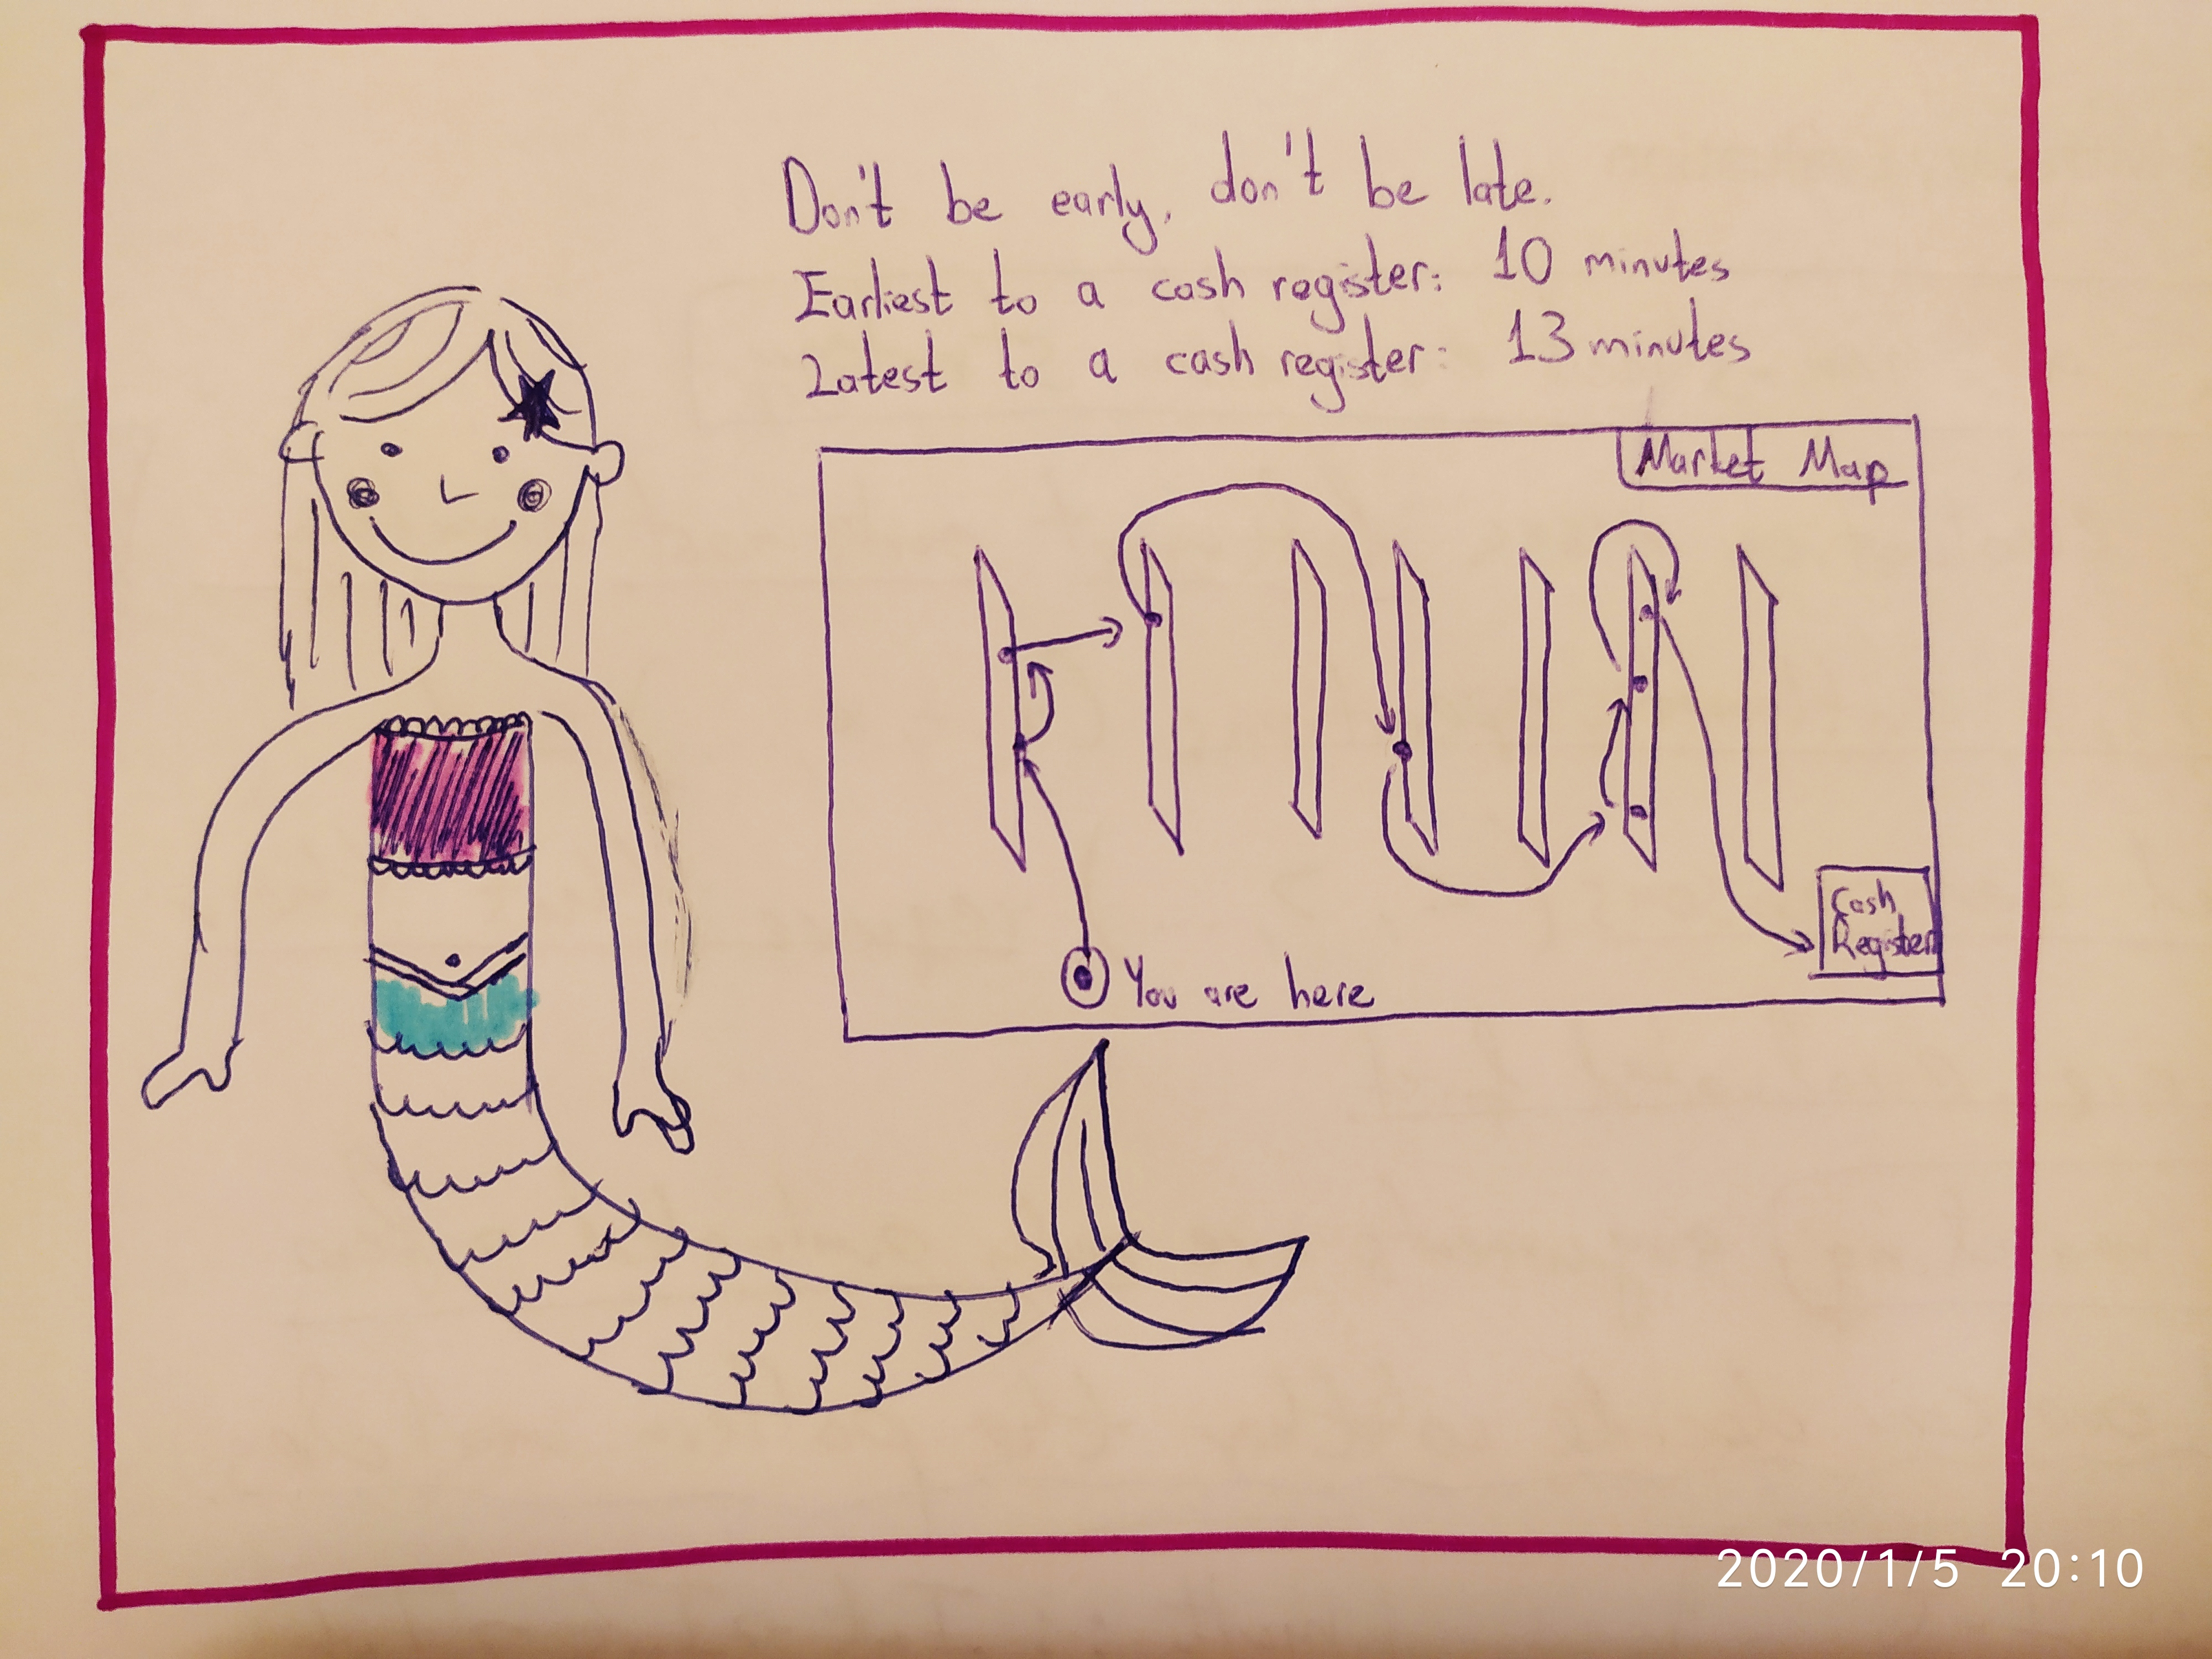
\includegraphics[width=0.8\textwidth, clip, trim={10em 8em 25em 0em}]{images/s2_p1.jpg}
	\caption{Solution \#2 Storyboard Update \#1: \newline Mascot amplified, the timeframe issue has been sorted}
\end{figure}
\begin{figure}[H]
	\centering
	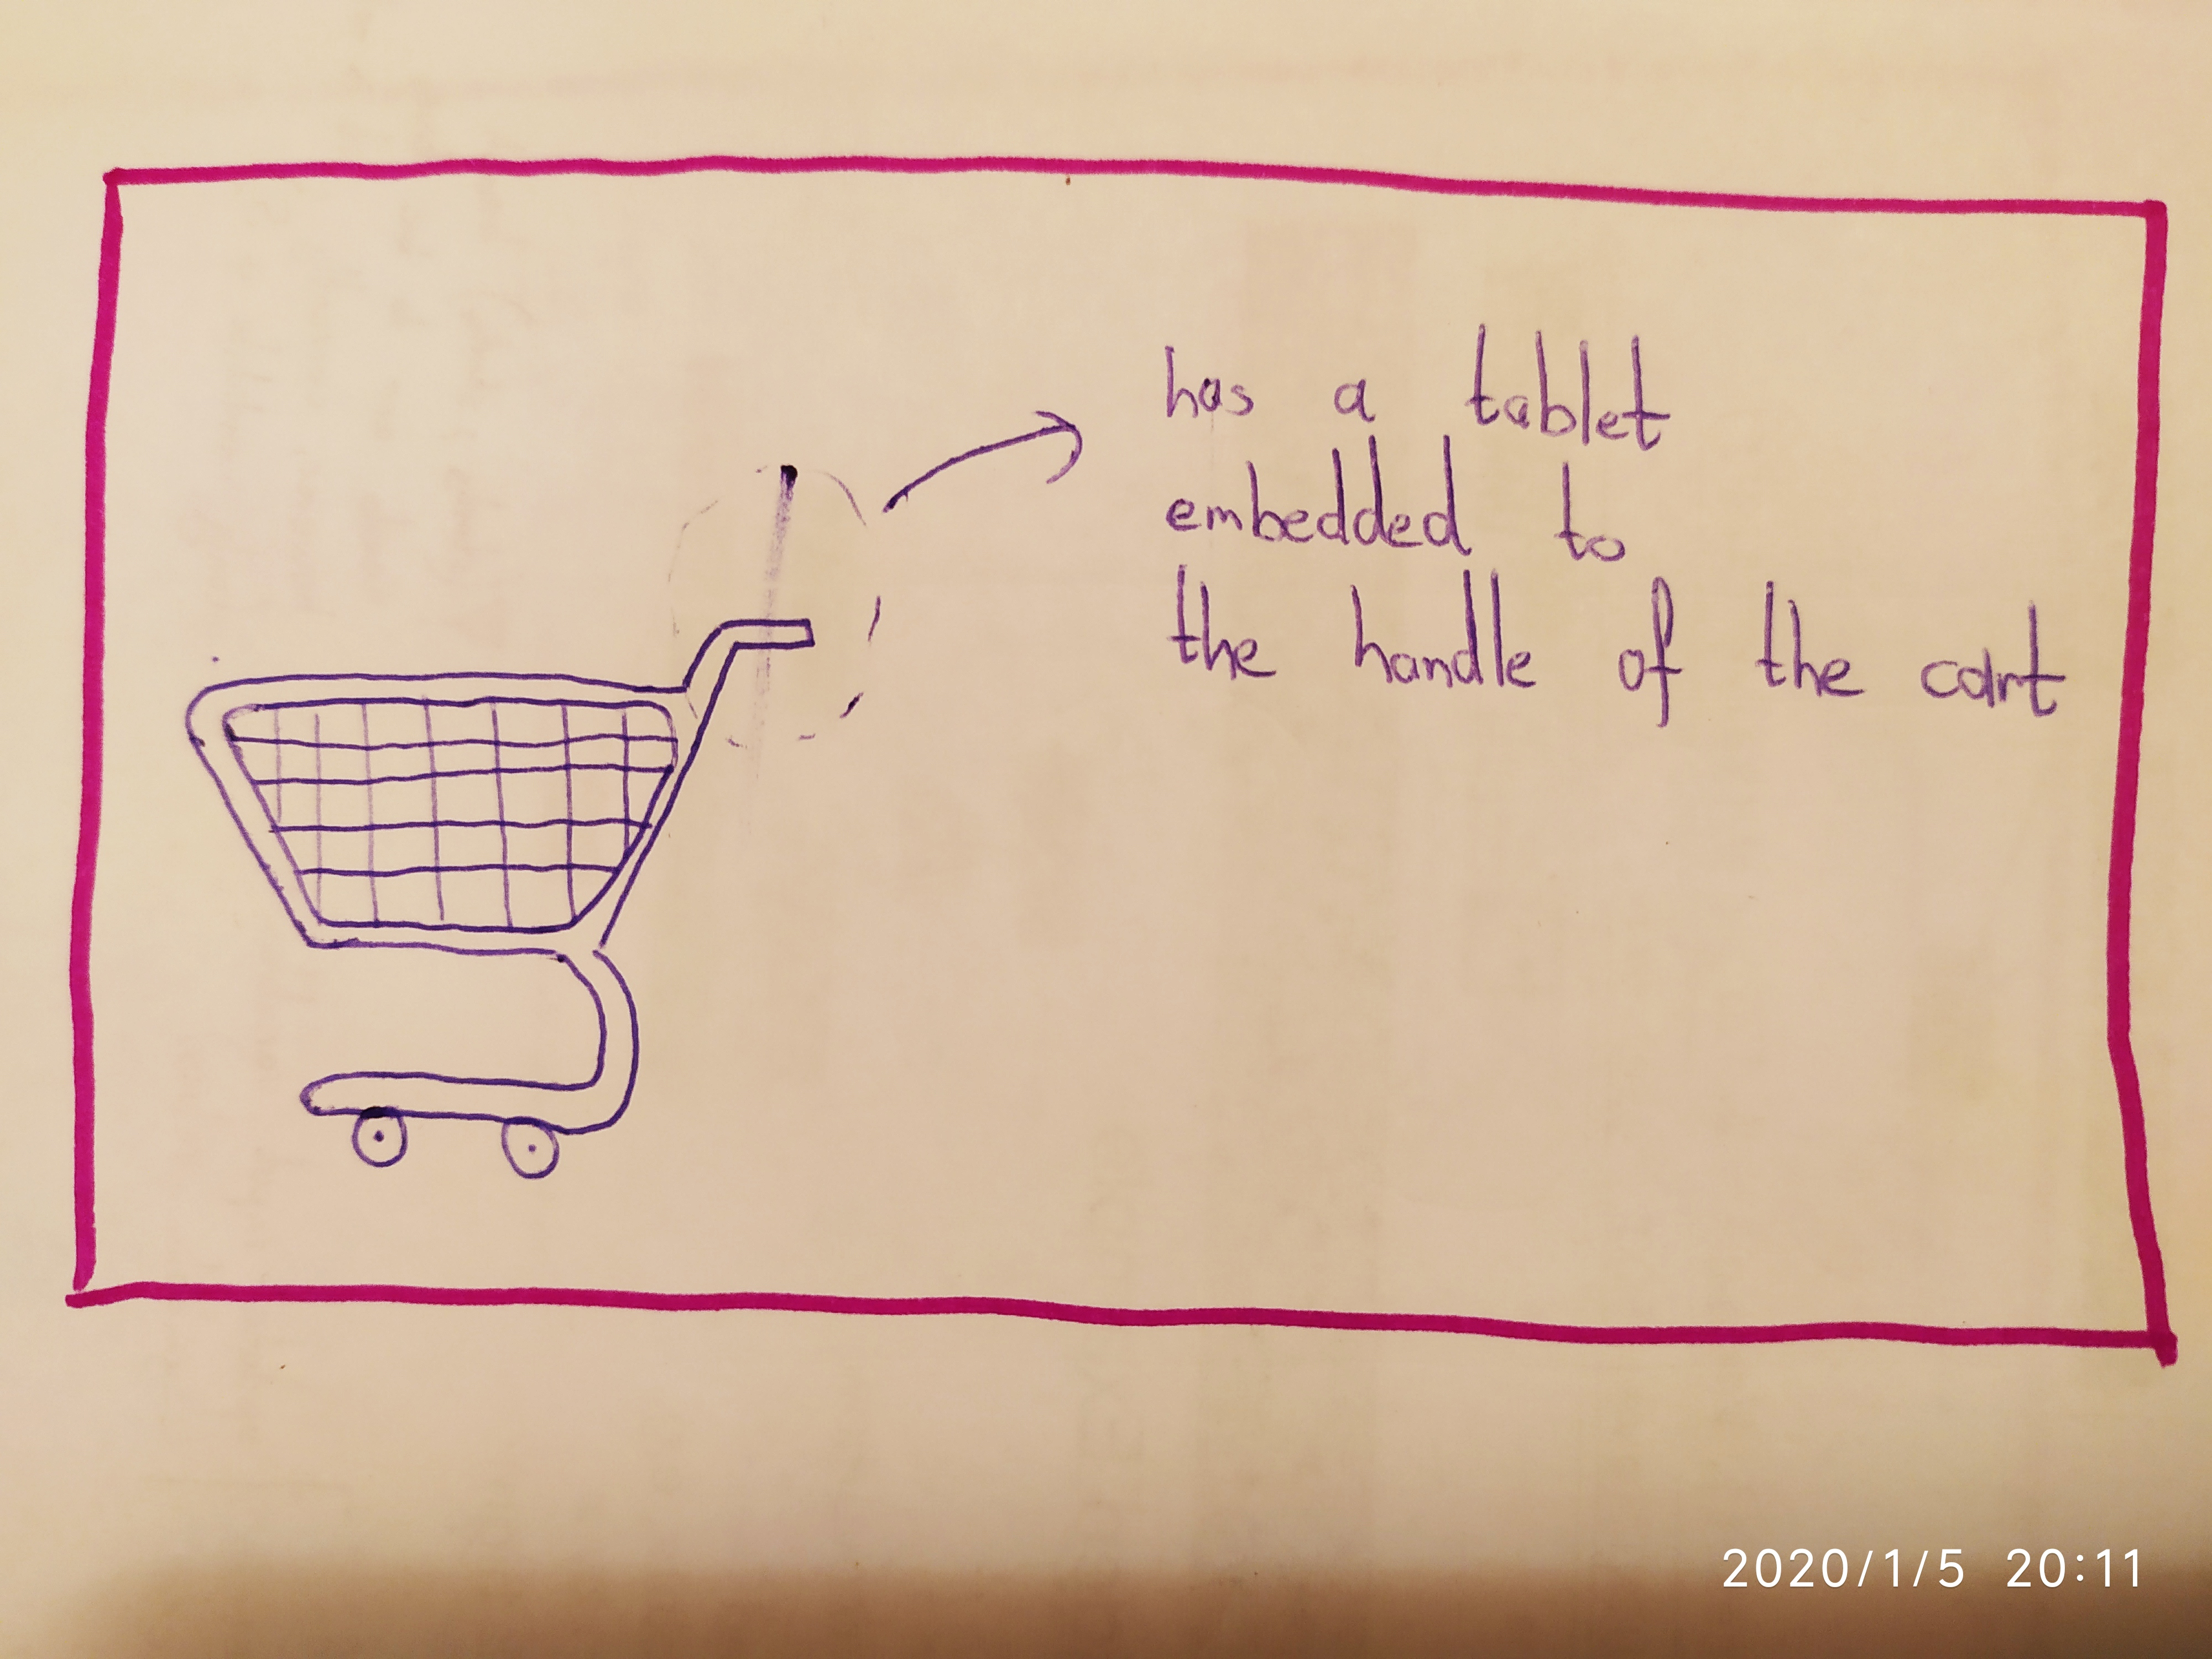
\includegraphics[width=0.8\textwidth, clip, trim={10em 50em 5em 20em}]{images/s2_p2.jpg}
	\caption{Solution \#2 Storyboard Update \#2: \newline The shopping cart + tablet relation explained in a more open sense}
\end{figure}
\bigskip
\bigskip
Note that these images would be embedded into the storyboards (avoided redrawing the whole storyboards).

\section{Solution \#y:}

\section{Solution \#z:}
				
\end{document}}
